% Options for packages loaded elsewhere
\PassOptionsToPackage{unicode}{hyperref}
\PassOptionsToPackage{hyphens}{url}
%
\documentclass[
]{article}
\usepackage{amsmath,amssymb}
\usepackage{lmodern}
\usepackage{iftex}
\ifPDFTeX
  \usepackage[T1]{fontenc}
  \usepackage[utf8]{inputenc}
  \usepackage{textcomp} % provide euro and other symbols
\else % if luatex or xetex
  \usepackage{unicode-math}
  \defaultfontfeatures{Scale=MatchLowercase}
  \defaultfontfeatures[\rmfamily]{Ligatures=TeX,Scale=1}
\fi
% Use upquote if available, for straight quotes in verbatim environments
\IfFileExists{upquote.sty}{\usepackage{upquote}}{}
\IfFileExists{microtype.sty}{% use microtype if available
  \usepackage[]{microtype}
  \UseMicrotypeSet[protrusion]{basicmath} % disable protrusion for tt fonts
}{}
\makeatletter
\@ifundefined{KOMAClassName}{% if non-KOMA class
  \IfFileExists{parskip.sty}{%
    \usepackage{parskip}
  }{% else
    \setlength{\parindent}{0pt}
    \setlength{\parskip}{6pt plus 2pt minus 1pt}}
}{% if KOMA class
  \KOMAoptions{parskip=half}}
\makeatother
\usepackage{xcolor}
\usepackage[margin=1in]{geometry}
\usepackage{graphicx}
\makeatletter
\def\maxwidth{\ifdim\Gin@nat@width>\linewidth\linewidth\else\Gin@nat@width\fi}
\def\maxheight{\ifdim\Gin@nat@height>\textheight\textheight\else\Gin@nat@height\fi}
\makeatother
% Scale images if necessary, so that they will not overflow the page
% margins by default, and it is still possible to overwrite the defaults
% using explicit options in \includegraphics[width, height, ...]{}
\setkeys{Gin}{width=\maxwidth,height=\maxheight,keepaspectratio}
% Set default figure placement to htbp
\makeatletter
\def\fps@figure{htbp}
\makeatother
\setlength{\emergencystretch}{3em} % prevent overfull lines
\providecommand{\tightlist}{%
  \setlength{\itemsep}{0pt}\setlength{\parskip}{0pt}}
\setcounter{secnumdepth}{-\maxdimen} % remove section numbering
\newlength{\cslhangindent}
\setlength{\cslhangindent}{1.5em}
\newlength{\csllabelwidth}
\setlength{\csllabelwidth}{3em}
\newlength{\cslentryspacingunit} % times entry-spacing
\setlength{\cslentryspacingunit}{\parskip}
\newenvironment{CSLReferences}[2] % #1 hanging-ident, #2 entry spacing
 {% don't indent paragraphs
  \setlength{\parindent}{0pt}
  % turn on hanging indent if param 1 is 1
  \ifodd #1
  \let\oldpar\par
  \def\par{\hangindent=\cslhangindent\oldpar}
  \fi
  % set entry spacing
  \setlength{\parskip}{#2\cslentryspacingunit}
 }%
 {}
\usepackage{calc}
\newcommand{\CSLBlock}[1]{#1\hfill\break}
\newcommand{\CSLLeftMargin}[1]{\parbox[t]{\csllabelwidth}{#1}}
\newcommand{\CSLRightInline}[1]{\parbox[t]{\linewidth - \csllabelwidth}{#1}\break}
\newcommand{\CSLIndent}[1]{\hspace{\cslhangindent}#1}
\ifLuaTeX
  \usepackage{selnolig}  % disable illegal ligatures
\fi
\IfFileExists{bookmark.sty}{\usepackage{bookmark}}{\usepackage{hyperref}}
\IfFileExists{xurl.sty}{\usepackage{xurl}}{} % add URL line breaks if available
\urlstyle{same} % disable monospaced font for URLs
\hypersetup{
  pdftitle={Beyond compositionally in high throughput sequencing; estimating the importance of scale in data analysis with ALDEx2},
  hidelinks,
  pdfcreator={LaTeX via pandoc}}

\title{Beyond compositionally in high throughput sequencing; estimating
the importance of scale in data analysis with ALDEx2}
\author{Gregory B. Gloor$^1$ \and Michelle Pistner Nixon$^2$ \and Justin Silverman$^{2,3}$}
\date{\today}

\begin{document}
\maketitle

$^1$ Department of Biochemistry, University of Western Ontario
$^2$ College of Information Sciences and Technology, Pennsylvania  State University
$^3$ Department of Medicine, Pennsylvania  State University

\begin{abstract}
Despite scale being an important confounding variable, high throughput
sequencing generates data that are difficult to reconcile with the scale
of the underlying environment, but it has been shown that the scale of
the environment is related to the geometric mean of the parts of the
sample. The ALDEx2 R package builds a Bayesian model of the data and
here we report an update to the model that includes both random sampling
and scale estimates. We show that incorporating scale allows for robust
inference in a number of different experimental designs and we provide
guidance on how to incorporate scale inference into differential
abundance analysis. While all data normalizations in widespread use make
implicit assumptions about the scale of the system we suggest that
explicit rather than implicit scale models should be used.
\end{abstract}

\hypertarget{introduction}{%
\section{Introduction}\label{introduction}}

High throughput sequencing (HTS) is a universal tool to explore many
biological phenomenon such as gene expression (single-cell sequencing,
RNA-sequencing, meta-transcriptomics), microbial community composition
(16S rRNA gene sequencing, shotgun metagenomics) and differential enzyme
activity (selex, CRISPR killing). HTS proceeds by taking a fixed-number
sample from the environment, making a library, multiplexing (merging)
multiple libraries and applying a fixed number of molecules to the flow
cell. In essence it is a poll of the environment that is mixed with
other polls and then a poll of the mixture is taken. It should be clear
that the total number of molecules sequenced is driven by the capacity
of the instrument and not by the number of molecules in the sampled
environment(Lovell et al. 2015; Vandeputte et al. 2017; Props et al.
2017) .

Data that are generated by sequencing come from systems where scale is
usually important and may be a confounding variable (Lovell et al.
2015). For example, cells transformed by the cMyc oncogene have about 3
times the amount of mRNA and about twice the rRNA content than do
non-transformed cells (Nie et al. 2012), and this dramatically skews
transcriptome analysis (Lovén et al. 2012). In addition, wild-type and
mutant strains of cell lines, yeast or bacteria often have different
growth rates, which would affect our ability to identify truly
differentially abundant genes (Yoshikawa et al. 2011). As another
example, the total bacterial load of the vaginal microbiome differs by
1-2 orders of magnitude in absolute abundance between the healthy and
bacterial vaginosis states (Zozaya-Hinchliffe et al. 2010); the
composition is dramatically different as well (Ravel et al. 2011;
Hummelen et al. 2010). Thus, the full description of these systems
includes both relative change (composition) and absolute abundance
(scale) but current methods access only the compositional information.

More formally, if the true information in the environment being sampled
can be summarized by counts of features (genes, taxa, etc) in a matrix
\(\mathbf{W}\), then the elements of the matrix can be decomposed into
its composition (relative information, \(\mathbf{W}^{\parallel}\) ) and
its scale (total sum, \(\mathbf{W}^{\perp}\) ); formally,
\(\mathbf{W} = \mathbf{W}^{\parallel} \mathbf{W}^{\perp}\). If the
matrix has \(N\) samples and \(D\) parts, then we can uniquely identify
\(\mathbf{W}_{dn}\) as the \(d^{th}\) feature in sample \(n\). Any data
that we collect by sequencing is thought to contain only proportional
(Lovell et al. 2011) information and we can represent the corresponding
sequenced matrix as \(\mathbf{Y}\). Compositional data analysis makes
the strong assumption that
\(\mathbf{Y}_{n} \equiv \mathbf{Y}^{\parallel}_{n} = f(\mathbf{W}^{\parallel}_{n})\);
in other words that what is measured by sequencing is relative
information only, and that this measurement is a function of the
relative information in the underlying environment. Note that under this
assumption no corresponding estimate or information is available for the
scale of the sample \(\mathbf{Y}^{\perp}_{n}\).

One issue that was realized very early was that if the goal was to
compare one sample to another then the output from HTS needed to be
normalized in order to make the samples commensurate and to correct any
minor asymmetries in the data. A large number of normalizations were
developed. Rarefaction(Hughes and Hellmann 2005) was used in the
microbiome field, while transcriptome investigators developed and used
proportions and derivatives (reads per kilobase per million, and
transcripts per kilobase per million(Mortazavi et al. 2008; Wagner, Kin,
and Lynch 2012)), the relative log expression (RLE)(Anders and Huber
2010) and trimmed mean of M values (TMM)(Robinson and Oshlack 2010). The
centered log ratio (CLR)(Aitchison 1982) approach was proposed as a
unifying normalization(Fernandes et al. 2014). With the exception of
rarefaction, all of these normalizations are ratios with the major
differences between approaches being how the denominator is chosen and
whether the ratio is always log transformed or not.

Recently, Nixon et al. (2023) showed that that \emph{all} normalizations
make some identifying assumption about the scale of \(\mathbf{W}\) but
that the actual assumption being made was not always easy to interpret.
In essence, normalizations in widespread use assume that either one
sample can be chosen as a reference to which the others are scaled
(TMM), or that different sub-parts of each sample maintain a constant
scale across samples (RLE, CSS, CLR and derivatives).

The CLR, which can be written as
\(\mathbf{CLR}_{(1...d)n} = \mathbf{Y}_{(1...d)n} / G_n\), uses the
geometric mean \(G_n\) of \(\mathbf{Y}^{\parallel}_{n}\) to scale the
data. Nixon et al. (2023) discovered that using the CLR was equivalent
to making a statement that \(G_n\) was related to the scale of the
underlying environment \(\mathbf{W}^{\perp}\). Interestingly, the
information in a system is a fundamental property and \(G_n\) is
strongly correlated with Shannon's entropy, indicating that information
about the complexity of \(\mathbf{W}\) is available post-sequencing
(Supplemental). The realization that all normalizations made assumptions
of scale led to the understanding that all normalizations introduced
latent bias into analyses because the scaling factor has been assumed up
to now to be a perfect point estimate of the scale of the underlying
system (Nixon et al. 2023).

With this new insight Nixon et al. (2023) devised methods to set up a
scale model that explicitly acknowledges and accounts for the
uncertainty of the scale. In the case of the CLR which uses the \(G_n\)
as the denominator, this entails adding uncertainty into \(G_n\) such
that the latent bias can be exposed, acknowledged and accounted for.
Additionally it was realized that the actual values used in the
denominator to calculate the log-ratio were irrelevant, but instead that
the ratios between the denominators was the key parameter. These two
insights allow for a full scale model of scale to be built and tested
for its effect on analysis.

The ALDEx2 R package (Fernandes et al. 2013) represents a general
purpose toolbox for Bayesian estimation of HTS datasets. ALDEx2 was
designed originally to convert the discrete point estimates in the count
matrix obtained into continuous posterior distributions through
Monte-Carlo sampling from the Dirichlet distribution. The posterior more
accurately represents variation on a per-sample basis(Gloor et al. 2016)
and this \(\mathbf{Y}^{\parallel}_{dn}\) can more closely approximate
\(\mathbf{W}^{\parallel}_{dn}\). Each Monte-Carlo replicate is
normalized using the CLR and used to calculate summary and test
statistics, and finally expected values and confidence intervals are
reported across the Monte-Carlo replicates. The CLR calculation can be
modified trivially to include a full scale model of the data by
incorporating uncertainty into \(G\) and so produce a posterior estimate
of the scale. The scale uncertainty can be included on a per-experiment,
per-group or even a per-sample basis. Thus, ALDEx2 can now be used to
generate a full posterior model of both \(\mathbf{W}^{\parallel}_{dn}\)
and \(\mathbf{W}^{\perp}_{dn}\) from the observed data.

An advantage of incorporating scale is that analyses can be made much
more robust such that actual or potential differences in scale can be
tested and accounted for explicitly. The examples below and in the
supplement show how incorporating scale provides robust and
interpretable differential abundance estimates in several different
datasets.

\hypertarget{results}{%
\section{Results}\label{results}}

The first dataset is a highly replicated yeast transcriptome where one
condition is wild-type and the other has a snf-1 gene
knockout(Gierliński et al. 2015). Yeast deficient for snf-1 grow more
slowly and are sensitive to a variety of common agents that cause cell
stress (Yoshikawa et al. 2011). This dataset has been used to argue that
only a small number of replicates need to be used to identity
differentially abundant genes and that different tools should be used
for datasets with different sample sizes because the tools have
different intrinsic statistical power and Type 1 and Type 2 errors
(Schurch et al. 2016). This guidance runs counter to standard
statistical practice where power is intrinsically linked to sample size
(Halsey et al. 2015), yet the concept of sample-size independent power
is entrenched in all fields that use HTS as an experimental readout.
Increasing false precision with increasing sample size can be understood
as the result of unacknowledged bias brought about because of false
certainty as to the scale of the data. Thus, by adding scale uncertainty
we can be more confident that the analysis is not converging on a
precise but biased estimate of scale (Gustafson 2015).

We start by examining the dispersion or variance of the data as counts
and as the logarithm of the normalized counts as calculated by DESeq2
(log(RLE)) and by ALDEx2 (CLR). The actual counts of data derived from
sequencing are overdispersed with the mean value being less than the
variance (Robinson, McCarthy, and Smyth 2010) as seen in Panel A of
Figure 1. This relationship is why most tools model the counts with the
Negative Binomial distribution(Frazee et al. 2023), and use this
distribution as the basis for batch correction(Zhang, Parmigiani, and
Johnson 2020). However, the actual analysis of differential abundance is
performed on the logarithm of the normalized counts (Robinson, McCarthy,
and Smyth 2010; Love, Huber, and Anders 2014; Andrews and Hemberg 2019),
or on the clr values (Fernandes et al. 2013) both of which are
log-ratios. The mean-dispersion distribution of these log-ratio
transformed data is quite different as shown in panels B and C of Figure
1 and as noted elsewhere (Fernandes et al. 2013; Love, Huber, and Anders
2014).

\begin{figure}
\centering
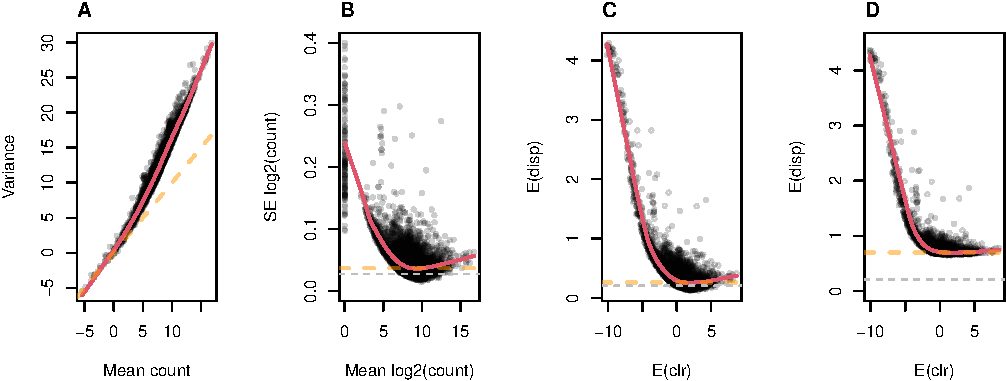
\includegraphics{go3_files/figure-latex/dispersion-1.pdf}
\caption{Plot of abundance v dispersion for a typical transcriptome
dataset as counts, as logarithms of counts, and as clr values. Panel A
shows that the data are over-dispersed relative to a Poisson
distribution which is represented by the dashed line when plotted on a
log-log scale. Panel B shows that the relationship between the mean and
the dispersion calculated in DESeq2, here the standard error (SE) of the
mean, is very different when the data are log-transformed first. Panel C
shows the equivalent values calculated by ALDEx2 in which the expected
clr value for each transcipt are plotted vs.~the expected dispersion.
The red line in each panel shows the loess line of fit to the mid-point
of the distributions. In panels B and C the amount of dispersion reaches
a minimum at moderate values. The dashed orange line in panel A is the
line of equivalence, and in panel B and C is the minimum y value. The
values below the dashed grey line in panels B and C represent those
below the first decile of dispersion.}
\end{figure}

Here we can see that while the variance or dispersion always increases
with increasing raw read count, it actually decreases when measured on
the log-ratio transformed data (Fernandes et al. 2013; Love, Huber, and
Anders 2014) and reaches a minimum at some mid-point of the
distribution. This makes the counter-intuitive suggestion that genes
with moderate expression have more predictable expression than genes
with very high expression such as housekeeping genes. This is at odds
with the known biology of cells where single cell counting of
housekeeping transcripts shows that they are both highly expressed and
have little intrinsic variation (Taniguchi et al. 2010). Furthermore,
the actual amount of dispersion is very small and for many transcripts
is almost negligible. To show this point more clearly, the majority of
the transcripts in the lowest decile of dispersion indicated below the
dashed grey line are statistically significantly different (75\% with
DESeq2, 69\% with ALDEx2), suggesting that low dispersion estimates lead
to many false positives because of the underestimation of dispersion.
The work of Nixon et al. (2023) suggests that this is because the biased
scale estimates that are calculated. Thus, the actual variation of
highly expressed genes is not captured accurately by current approaches
to analysis and supports the idea that HTS have unacknowledged bias.

Using either DESeq2 or ALDEx2, we observe that a majority of transcripts
are statistically significantly different between groups even with a
Benjamini-Hochberg (Benjamini and Hochberg 1995) false discovery rate
(FDR) of 0.01; i.e.~4264 or 3790 of the 5891 transcripts are
statistically significant. Clearly, the necessary assumption of most
features being invariant is not justified. Applying the rule of thumb of
at least a \(2^{1.4}\) fold change (Schurch et al. 2016) reduces these
outputs to 193 for DESeq2 and to 186 for ALDEx2.

\begin{figure}
\centering
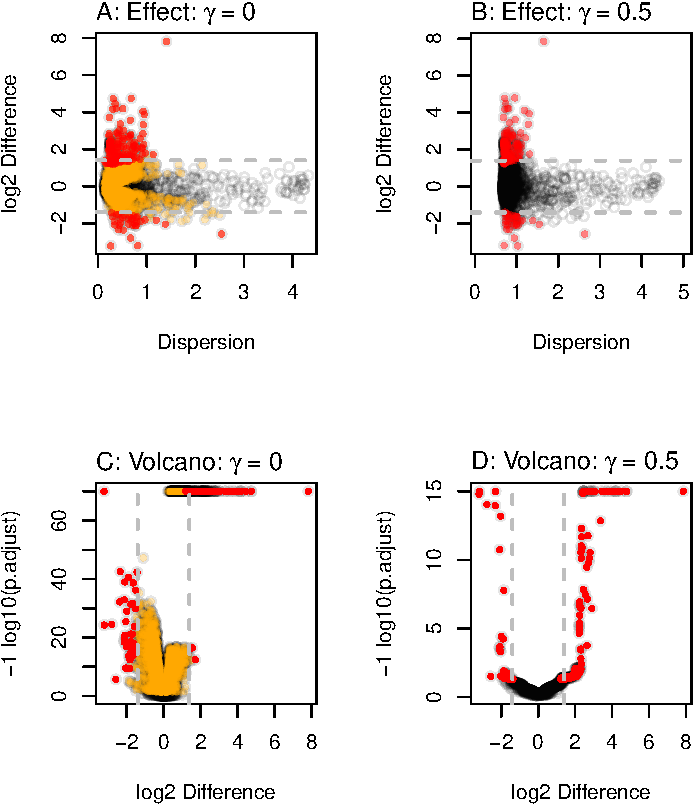
\includegraphics{go3_files/figure-latex/plot1-1.pdf}
\caption{Effect and volcano plots for unscaled and scaled transcriptome
analysis. DESeq2 or ALDEx2 were used to conduct a differential abundance
(DA) analysis on the yeast transcriptome dataset. The results were
plotted to show the relationship between difference and dispersion using
effect plots ) or difference and the Benjamini-Hochberg corrected
p-values (volcano plot). Panels A,B,D,E are for the unscaled analysis,
and Panels C,F are for the scaled analysis. Each point represents the
values for one transcript, with the color indicating if that transcript
was significant in the scaled analysis and unscaled analysis (red) or in
the unscaled analysis only (orange). Points in grey are not
statistically signficantly different with any analysis. The horizontal
dashed lines represent a log2(difference) of 1.4, which is a commonly
applied cutoff when the majority of features are statistically
significant.}
\end{figure}

As shown using the effect (Gloor, Macklaim, and Fernandes 2016) and
volcano plots (Cui and Churchill 2003) in Figure 2 A,B,D,E the root
cause of the many statistically significant positive transcripts is the
very large number of transcripts with negligible variance with both
DESeq2 and ALDEx2. We can see that almost all the transcripts that are
differentially abundant with an FDR \textless{} 0.01 (orange and red
points) have extremely low dispersion and a very low difference between
groups. In the most extreme cases transcripts with near 0 difference
have a low FDR. This issue lead to the common practice of choosing
transcripts with a low FDR and a fold-change threshold (Schurch et al.
2016) (commonly set at \(\pm 2^{1.4}\)), and these limits are shown by
the dashed grey lines. A similar sitation arises when using the ALDEx2
package, and indeed the two methods identify substantially similar
transcripts. This results begs the question, ``why bother with the
signficance test?''.

The very low dispersion estimate for most of the features arises because
scale variation in the underlying dataset has been removed through
sequencing and normalization. While the actual scale of the data is
inaccessible post-sequencing we can estimate the \emph{effect} of scale
on the output. To do this, we add uncertainty to the denominator that is
used to calculate the log-ratio of the samples (Nixon et al. 2023), and
combine this with the posterior probabilities that ALDEx2 calculates on
a per-feature basis (Fernandes et al. 2013). Scale uncertainty is
incorporated using the \texttt{gamma} parameter that controls the amount
uncertainty being included when we call either \texttt{aldex()}, or
\texttt{aldex.clr()}. The \texttt{ALDEx2} package further contains a
sensitivity analysis function, \texttt{aldex.senAnalysis()}, that can be
used to explore the effect of different amounts of scale uncertainty. In
practice we suggest that a \texttt{gamma} parameter between 0.5 and 1 is
realistic for most experimental designs.

Applying \texttt{gamma=1} as a parameter we can see that the large
number of transcripts with near 0 dispersion have had their dispersion
increased (Figure 2C), and this results in many fewer transcripts (100)
being called significantly different as shown in the volcano plot in
Figure 1F (red points). Furthermore, overplotting the significant
transcripts identified after adding scale uncertainty on the un-scaled
analysis shows that adding scale uncertainty removes the need for the
dual cutoff. Indeed, adding scale uncertainty reduces the significant
transcripts to approximately the number observed with the somewhat
arbitrary difference cutoff. Thus, incorporating scale uncertainty
through the default scale model allows us to determine which variables
are likely to be significant due to sequencing and normalization, and
which are significantly different even with scale uncertainty included.

The second example dataset is a vaginal metatranscriptome dataset used
in (Macklaim and Gloor 2018; Wu et al. 2021), where we are comparing
gene expression in bacteria collected from healthy (H) and bacterial
vaginosis (BV) affected women. In this environment, both the relative
abundance of species between groups is different as is the gene
expression levels within a species (Macklaim et al. 2013). We further
know that the total number of bacteria is about 10X more in BV than in H
(Zozaya-Hinchliffe et al. 2010). Thus, this is an extremely challenging
environment in which to determine differential abundance. Indeed, the
accepted method to not analyze the vaginal metatranscriptome as a whole
system but instead to do the simpler taxon-by-taxon (Macklaim et al.
2013; Deng et al. 2018; Fettweis et al. 2019). The problem with the
systemic analysis is that the scale confounding results in many
housekeeping genes as being differentially abundant between groups.

In this example we show how to specify the scale model explicitly and
demonstrate that applying different scale models to each group
independently can control for the very large difference in scale in the
underlying data. When specifying the whole scale model we can pass a
matrix of scale values instead of a single estimate of gamma to
\texttt{aldex.clr()}. This matrix should have the same number of rows as
the of Monte-Carlo Dirichlet samples, and the same number of columns as
the number of samples. There is an \texttt{aldex.makeScaleModel()}
function that can be used to simplify this step.

This scale model matrix encapsulates two aspects of scale uncertainty
and explicitly illustrates the concept of scale. First, as in the first
example, the gamma paramter indicates the scale uncertainty. Second, we
need to explicitly indicate the difference in scale between the groups
in the dataset.

Figure 3A shows an effect plot (Gloor, Macklaim, and Fernandes 2016) of
the data where reads are grouped by function, corresponding
approximately to grouping orthologous sequences regardless of the
organism of origin. Each point represents one of the 3728 functions, and
we can see that there are many more functions represented in the BV
group (bottom) than in the healthy group (top). This is because the
\textit{Lactobacilli} that dominate a healthy vaginal microbiome have
reduced genome content relative to the anaerobic organisms that dominate
in BV, because there is a greater diversity of organisms in BV than in H
samples and because the BV condition has at least an order of magnitude
more bacteria than does the H condition.

We can see that there are a large number of functions that are shared
between the two groups (boxed area in Figure 3A), and inspection shows
that these largely correspond to core metabolic functions that would not
be expected to contribute to differences in ecosystem behaviour. As a
proxy for housekeeping functions the core ribosome functions (blue)
shows that their mean location is not centred on 0. The major group of
these housekeeping functions is located off the line of no difference
(being approximately located at +1.5) and not surprisingly have among
the lowest dispersion in the dataset. Nevertheless, they are identified
as differentially abundant (red) along with many others. While changes
in the abundance of housekeeping functions is a useful proxy for
relative abundance of species in the environment, they tell us nothing
about the functional capacity of the two groups because these are
functions in common to every organism. Of more interest is determining
the functions that are different between groups because these are unique
or over-expressed in one group relative to the other.

\begin{figure}
\centering
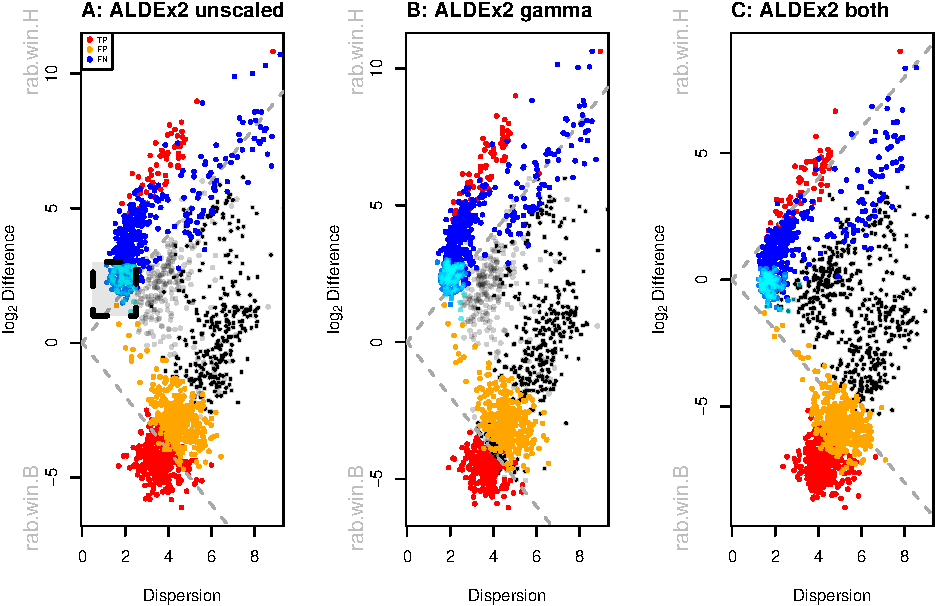
\includegraphics{go3_files/figure-latex/meta-1.pdf}
\caption{Analysis of vaginal transcriptome data aggregated at the Kegg
Orthology (KO) functional level. Panel A shows an effect plot for the
default analysis where the functions that are elevated in the healthy
individuals have positive values and functions that are elevated in BV
have negative values. Highlighed in the box are highly abundant KOs that
are almost exlusively housekeeping functions, with ribosomal KOs
highlighted in blue, statistically significant (FDR \textless{} 0.01)
functions in red, and non-significant functions in black or orange.
These housekeeping functions should be located on the midline of no
difference. Panel B shows the same data scaled with
\texttt{gamma\ =\ 1}, which increase the minimum dispersion approximatly
by one unit. Here the housekeeping functions from Panel A are colored
cyan or blue for reference. Panel C shows the same data scaled with
\texttt{gamma\ =\ 0.75} and a 0.15 fold difference in dispersion applied
to the BV samples relative to the H samples. The orange functions are
now statistically significant. Note that this shifts the midpoint of the
housekeeping functions towards the midline.}
\end{figure}

Applying the default scale model of \texttt{gamma=1} as before increases
the dispersion as expected, but does little to move the large number of
housekeeping functions toward the midline of no difference.
Nevertheless, about 50\% of the housekeeping functions are no longer
statistically significantly different.

Up to this point, scale uncertainty has been applied uniformly to both
conditions, but a user-defined scale adjustment can be applied to each
condition, or even each sample independently through a custom scale
matrix. For this we need to revisit the concept that all normalizations
in widespread use are actually ratios with the denominator chosen by one
of several methods. It is important to recognize that in some datasets
the denominator itself is not crucial as all approaches give
substantially similar results; the transcriptome example used previously
is a good example of such an idealized dataset. This begs the question,
``if it is not the denominator, what then is the important
determinant?'' As shown by Nixon et al. (2023) it is usually the
\emph{relationship} between the group scale values (denominators) that
is important, not their actual value. This can be illustrated quite
simply by starting with the mean ratio in \(G\) between groups for the
yeast transcriptome dataset which are \(6.05\times^{-5}\) for snf-w and
\(5.08\times^{-5}\); their ratio being 1.17, or a 0.17-fold difference.
Using this information, we can recapitulate the differential abundance
analysis in Figure 2B and 2C exactly by using setting the mean
denominator of group 1 to 1, and group 2 to 1.17 with a gamma of 1 as
shown in Supplemental Figure 2. Altering this ratio moves the location
of the data.

With this background, we can understand how to apply a full scale to the
metatranscriptome dataset with the \texttt{aldex.makeScaleMatrix()}
function. This function uses a logNormal distribution when building the
model so that ratios that are chosen are symmetrical. The full scale
model option can be used to make a matrix of relative scales that are
distinct for each group (or even each sample) along with their
uncertainties. Applying a per-group relative differential scale of 0.15
with a base scale of 1 moves the housekeeping functions to the midline
of no difference (Figure 3C). Note that now a significant number of
functions are differentially up in BV that were formerly classed as not
different without scale, or when only a uniform scale was applied. These
former false negatives are noted in orange in each panel. Inspection of
the functions shows that these are largely missing from the
Lactobacillus species and so should actually be captured as
differentially abundant. Thus, applying differential scale allows us to
distinguish between both false positives (housekeeping functions in
cyan) and false negatives (orange functions) even in a very difficult to
analyze dataset. We suggest that the default scale model alone is useful
and should be normally applied when the data are well centred. However,
when datasets are not well centred or when the investigator has prior
information about the underlying biology, we advocate developing and
using a full differential scale model.

\hypertarget{discussion}{%
\section{Discussion}\label{discussion}}

Biological count data derived from HTS can be decomposed into two parts
the relative (compositional) and the absolute (scale), and the product
of these generates a fully scaled biological system (Nixon et al. 2023).
Biological systems are both predictably variable and stochastic and
current measurement methods that rely on high throughput sequencing fail
to capture all of that variation. In the absence of information external
to the sequencing run itself, no normalisation method can recapture any
of the scale information (Lovén et al. 2012).

Since the underlying scale of the system cannot be measured easily --
methods such as flow cytometry (Vandeputte et al. 2017), spike-in probes
and fluorescent in-situ hybridization (Lovén et al. 2012; Marguerat et
al. 2012) have been used -- the effect on analysis can be modelled by
including scale uncertainty in the analysis (Nixon et al. 2023). Nixon
et al, showed that this can be done by including uncertainty in the
denominator used for the normalization. The ALDEx2 R package is ideally
suited for this since this tool builds a Bayesian posterior of the
compositional component of the dataset at the outset and then conducts
the analysis on that posterior. Adding scale uncertainty can be done at
the same time thus producing a posterior model that incorporates both
compositional and scale uncertainty, and this can be done without
additional computational complexity. For this, the compositional
uncertainty is sampled from a Dirichlet distribution, and the scale
uncertainty can be sampled from any distribution depending on prior
knowledge or preference, but ALDEx2 samples from a logNormal
distribution by default.

All normalizations attempt to make the samples in a dataset commensurate
but do not explicitly address the scale of the underlying system. The
two supplementary tables show that these normalizations can be
interpreted as scale assumptions. However, the general lack of scale
information has important consequences for the analysis of HTS datasets.
One issue is that analysis tools seem over-powered with even moderate
sample sizes and different tools have different intrinsic power, Type 1
and Type 2 error rates (Schurch et al. 2016). Using small sample sizes
in analysis leads to less reliability and reproducibility in analyses
since surprisingly large sample sizes are needed to determine
reproducible p-values (eg. (Halsey et al. 2015)). Thus, recommendations
to use small sample sizes in multivariate datasets such as RNA-seq
datasets are not supported by simple modelling in the univariate case.
Another issue is that datasets are difficult to analyze when there they
contain systematic asymmetry, with different tools exhibiting differing
pathologies with these datasets (Robinson and Oshlack 2010; Wu et al.
2021).

Many groups have conducted benchmarking studies on different tools and
normalizations used for the analysis of datasets such as transcriptomes
(Bullard et al. 2010; Soneson and Delorenzi 2013; Schurch et al. 2016;
Quinn, Crowley, and Richardson 2018) and microbiomes(Thorsen et al.
2016; Weiss et al. 2017; Hawinkel et al. 2018). Generically, it is
observed that the actual agreement between methods can be modest, and
there is usually a recommendation that some methods are better suited
for individual datasets or for specific types of analysis;
e.g.~`Normalization and microbial differential abundance strategies
depend upon data characteristics' (Weiss et al. 2017). However, another
interpretation of these studies is that the specific assumptions of the
tools and the way they are used by different groups can lead to results
that include both false negative and false positive results, skewed
towards the latter. There are now published examples of multiple large
replication efforts in psychology (Open Science Collaboration 2015),
cancer biology (Rodgers and Collings 2021), ecology and evolution (Gould
and et.al, n.d.). In a nutshell, experiences from these studies indicate
that published data typically have higher effect sizes and appear more
significant than replication efforts with the same data, or with newly
generated replication data (Rodgers and Collings 2021). Thus, most
published data should be viewed with suspicion (Ioannidis 2005) unless
efforts have been made to ensure that the results are robust

In the case of overpowering, HTS analyses seem to be more robust when
applying a dual cutoff of both p-value and difference between group
means (Schurch et al. 2016). Figure 2 shows one reason for this
robustness could be that the dual cutoff is mimicking the effect of
including scale uncertainty, since substantially similar transcripts are
identified by the two approaches. However, while using the post-hoc
difference cutoff is useful for differential abundance analysis it is
not clear how this can be incorporated into other kinds of downstream
analyses. Conversely analyses that include scale uncertainty are fully
compatible with existing downstream analyses.

In the case of asymmetry, the use of a user-specified scale model can be
very useful for otherwise difficult to analyze datasets such as
meta-transcriptomes and in-vitro selection datasets where the majority
of features can change. We showed one such example in Figure 3 where the
dataset was highly asymmetrical, and the TMM and RLE normalizations
cannot fully move all the housekeeping genes to the midline of no
difference or exhibit other pathologies (supplemental). Incorporating
differential scale on a per-group basis moves the mass of the data
towards the midline of no difference and so affects both Type I and Type
II error rates. In this analysis, transcripts that were previously not
classed as differentially abundant are now called as significantly
different, and the housekeeping transcripts move from being
significantly different to not being identified as such. While we
acknowledge that some prior information on which housekeeping
transcripts should not be classed as DA is needed, we suggest that this
information is widely available and is already used when performing the
gold-standard quantitative PCR test of differential abundance (Thellin
et al. 1999; SEQC/MAQC-III Consortium 2014). Furthermore, the assumption
that housekeeping genes should not generally be included in differential
abundance analysis is implicit in the dual p-value, fold-change cutoff
approach in widespread use. Thus, the use of this prior knowledge is not
unique to our approach.

In summary, while the underlying scale of the system is generally
inaccessible, the effect of scale on the analysis outcomes can be
modelled and can help explain some of the underlying biology. Adding
scale information to the analysis allows for more robust inference
because the features that are sensitive to scale can be identified and
their impact on the analysis weighted accordingly. Additionally, the use
of differential scale models permits difficult to analyze datasets to be
examined in a robust and principled manner even when the majority of
features are asymmetrically distributed or expressed (or both) in the
groups. Thus, reporting scale uncertainty should become a standard
practice in the analysis of HTS datasets as a way to identify which
features are most robust to differences in the underlying system.
Finally, we supply a toolkit that makes incorporating scale simple even
for datasets that come from highly asymmetrical environments.

\hypertarget{refs}{}
\begin{CSLReferences}{1}{0}
\leavevmode\vadjust pre{\hypertarget{ref-aitchison1982}{}}%
Aitchison, John. 1982. {``The Statistical Analysis of Compositional
Data.''} \emph{Journal of the Royal Statistical Society: Series B
(Methodological)} 44 (2): 139--60.

\leavevmode\vadjust pre{\hypertarget{ref-Anders:2010}{}}%
Anders, Simon, and Wolfgang Huber. 2010. {``Differential Expression
Analysis for Sequence Count Data.''} \emph{Genome Biol} 11 (10): R106.
\url{https://doi.org/10.1186/gb-2010-11-10-r106}.

\leavevmode\vadjust pre{\hypertarget{ref-Andrews:2019aa}{}}%
Andrews, Tallulah S, and Martin Hemberg. 2019. {``M3Drop: Dropout-Based
Feature Selection for scRNASeq.''} \emph{Bioinformatics} 35 (16):
2865--67. \url{https://doi.org/10.1093/bioinformatics/bty1044}.

\leavevmode\vadjust pre{\hypertarget{ref-benjamini:1995}{}}%
Benjamini, Yoav, and Yosef Hochberg. 1995. {``Controlling the False
Discovery Rate: A Practical and Powerful Approach to Multiple
Testing.''} \emph{Journal of the Royal Statistical Society. Series B
(Methodological)} 57 (1): 289--300.

\leavevmode\vadjust pre{\hypertarget{ref-Bullard:2010}{}}%
Bullard, James H, Elizabeth Purdom, Kasper D Hansen, and Sandrine
Dudoit. 2010. {``Evaluation of Statistical Methods for Normalization and
Differential Expression in m{RNA-Seq} Experiments.''} \emph{BMC
Bioinformatics} 11: 94. \url{https://doi.org/10.1186/1471-2105-11-94}.

\leavevmode\vadjust pre{\hypertarget{ref-Cui:2003aa}{}}%
Cui, Xiangqin, and Gary A Churchill. 2003.
{``\href{https://www.ncbi.nlm.nih.gov/pubmed/12702200}{Statistical Tests
for Differential Expression in cDNA Microarray Experiments}.''}
\emph{Genome Biol} 4 (4): 210.1--10.

\leavevmode\vadjust pre{\hypertarget{ref-Denge00262-18}{}}%
Deng, Zhi-Luo, Cornelia Gottschick, Sabin Bhuju, Clarissa Masur,
Christoph Abels, and Irene Wagner-Döbler. 2018. {``Metatranscriptome
Analysis of the Vaginal Microbiota Reveals Potential Mechanisms for
Protection Against Metronidazole in Bacterial Vaginosis.''} Edited by
Craig D. Ellermeier, Janet Hill, and Andrew Onderdonk. \emph{mSphere} 3
(3). \url{https://doi.org/10.1128/mSphereDirect.00262-18}.

\leavevmode\vadjust pre{\hypertarget{ref-fernandes:2013}{}}%
Fernandes, Andrew D, Jean M Macklaim, Thomas G Linn, Gregor Reid, and
Gregory B Gloor. 2013. {``ANOVA-Like Differential Expression (ALDEx)
Analysis for Mixed Population RNA-Seq.''} \emph{PLoS One} 8 (7): e67019.
\url{https://doi.org/10.1371/journal.pone.0067019}.

\leavevmode\vadjust pre{\hypertarget{ref-fernandes:2014}{}}%
Fernandes, Andrew D, Jennifer Ns Reid, Jean M Macklaim, Thomas A
McMurrough, David R Edgell, and Gregory B Gloor. 2014. {``Unifying the
Analysis of High-Throughput Sequencing Datasets: Characterizing
{RNA}-Seq, 16{S} r{RNA} Gene Sequencing and Selective Growth Experiments
by Compositional Data Analysis.''} \emph{Microbiome} 2: 15.1--13.
\url{https://doi.org/10.1186/2049-2618-2-15}.

\leavevmode\vadjust pre{\hypertarget{ref-Fettweis:2019aa}{}}%
Fettweis, Jennifer M, Myrna G Serrano, J Paul Brooks, David J Edwards,
Philippe H Girerd, Hardik I Parikh, Bernice Huang, et al. 2019. {``The
Vaginal Microbiome and Preterm Birth.''} \emph{Nat Med} 25 (6):
1012--21. \url{https://doi.org/10.1038/s41591-019-0450-2}.

\leavevmode\vadjust pre{\hypertarget{ref-polyester:2016}{}}%
Frazee, Alyssa C., Andrew E. Jaffe, Rory Kirchner, and Jeffrey T. Leek.
2023. {``{polyester: Simulate RNA-seq reads}.''}
\url{https://doi.org/10.18129/B9.bioc.polyester}.

\leavevmode\vadjust pre{\hypertarget{ref-Gierlinski:2015aa}{}}%
Gierliński, Marek, Christian Cole, Pietà Schofield, Nicholas J Schurch,
Alexander Sherstnev, Vijender Singh, Nicola Wrobel, et al. 2015.
{``Statistical Models for RNA-Seq Data Derived from a Two-Condition
48-Replicate Experiment.''} \emph{Bioinformatics} 31 (22): 3625--30.
\url{https://doi.org/10.1093/bioinformatics/btv425}.

\leavevmode\vadjust pre{\hypertarget{ref-gloor:effect}{}}%
Gloor, GB, JM Macklaim, and AD Fernandes. 2016. {``Displaying Variation
in Large Datasets: Plotting a Visual Summary of Effect Sizes.''}
\emph{Journal of Computational and Graphical Statistics} 25 (3C):
971--79. \url{https://doi.org/10.1080/10618600.2015.1131161}.

\leavevmode\vadjust pre{\hypertarget{ref-gloorAJS:2016}{}}%
Gloor, GB, JM Macklaim, M Vu, and AD Fernandes. 2016. {``Compositional
Uncertainty Should Not Be Ignored in High-Throughput Sequencing Data
Analysis.''} \emph{Austrian Journal of Statistics} 45: 73--87.
\url{https://doi.org/doi:10.17713/ajs.v45i4.122}.

\leavevmode\vadjust pre{\hypertarget{ref-evoRepr-pre}{}}%
Gould, E, and et.al. n.d. {``Same Data, Different Analysts: Variation in
Effect Sizes Due to Analytical Decisions in Ecology and Evolutionary
Biology.''} \emph{EcoEvoRxiv}.
https://doi.org/\url{https://doi.org/10.32942/X2GG62}.

\leavevmode\vadjust pre{\hypertarget{ref-gustafson2015bayesian}{}}%
Gustafson, Paul. 2015. \emph{Bayesian Inference for Partially Identified
Models: Exploring the Limits of Limited Data}. Vol. 140. CRC Press.

\leavevmode\vadjust pre{\hypertarget{ref-Halsey:2015aa}{}}%
Halsey, Lewis G, Douglas Curran-Everett, Sarah L Vowler, and Gordon B
Drummond. 2015. {``The Fickle p Value Generates Irreproducible
Results.''} \emph{Nat Methods} 12 (3): 179--85.
\url{https://doi.org/10.1038/nmeth.3288}.

\leavevmode\vadjust pre{\hypertarget{ref-hawinkel2017}{}}%
Hawinkel, Stijn, Federico Mattiello, Luc Bijnens, and Olivier Thas.
2018. {``A Broken Promise : Microbiome Differential Abundance Methods Do
Not Control the False Discovery Rate.''} \emph{BRIEFINGS IN
BIOINFORMATICS}. \url{http://dx.doi.org/10.1093/bib/bbx104}.

\leavevmode\vadjust pre{\hypertarget{ref-Hughes:2005tu}{}}%
Hughes, Jennifer B, and Jessica J Hellmann. 2005. {``The Application of
Rarefaction Techniques to Molecular Inventories of Microbial
Diversity.''} \emph{Methods Enzymol} 397: 292--308.
\url{https://doi.org/10.1016/S0076-6879(05)97017-1}.

\leavevmode\vadjust pre{\hypertarget{ref-Hummelen:2010}{}}%
Hummelen, Ruben, Andrew D Fernandes, Jean M Macklaim, Russell J Dickson,
John Changalucha, Gregory B Gloor, and Gregor Reid. 2010. {``Deep
Sequencing of the Vaginal Microbiota of Women with {HIV}.''} \emph{PLoS
One} 5 (8): e12078. \url{https://doi.org/10.1371/journal.pone.0012078}.

\leavevmode\vadjust pre{\hypertarget{ref-Ioannidis:2005aa}{}}%
Ioannidis, John P A. 2005. {``Why Most Published Research Findings Are
False.''} \emph{PLoS Med} 2 (8): e124.
\url{https://doi.org/10.1371/journal.pmed.0020124}.

\leavevmode\vadjust pre{\hypertarget{ref-Love:2014aa}{}}%
Love, Michael I, Wolfgang Huber, and Simon Anders. 2014. {``Moderated
Estimation of Fold Change and Dispersion for RNA-Seq Data with
DESeq2.''} \emph{Genome Biol} 15 (12): 550.1--21.
\url{https://doi.org/10.1186/s13059-014-0550-8}.

\leavevmode\vadjust pre{\hypertarget{ref-lovell:2011}{}}%
Lovell, David, Warren Müller, Jen Taylor, Alec Zwart, and Chris
Helliwell. 2011. {``Proportions, Percentages, Ppm: Do the Molecular
Biosciences Treat Compositional Data Right?''} In \emph{Compositional
Data Analysis: Theory and Applications}, edited by Vera Pawlowsky-Glahn
and Antonella Buccianti, 193--207. London: John Wiley; Sons New York,
NY.

\leavevmode\vadjust pre{\hypertarget{ref-Lovell:2015}{}}%
Lovell, David, Vera Pawlowsky-Glahn, Juan José Egozcue, Samuel
Marguerat, and Jürg Bähler. 2015. {``Proportionality: A Valid
Alternative to Correlation for Relative Data.''} \emph{PLoS Comput Biol}
11 (3): e1004075.
https://doi.org/\url{https://doi.org/10.1371/journal.pcbi.1004075}.

\leavevmode\vadjust pre{\hypertarget{ref-Loven:2012aa}{}}%
Lovén, Jakob, David A Orlando, Alla A Sigova, Charles Y Lin, Peter B
Rahl, Christopher B Burge, David L Levens, Tong Ihn Lee, and Richard A
Young. 2012. {``Revisiting Global Gene Expression Analysis.''}
\emph{Cell} 151 (3): 476--82.
\url{https://doi.org/10.1016/j.cell.2012.10.012}.

\leavevmode\vadjust pre{\hypertarget{ref-macklaim:2013}{}}%
Macklaim, Jean M, Andrew D Fernandes, Julia M Di Bella, Jo-Anne Hammond,
Gregor Reid, and Gregory B Gloor. 2013. {``Comparative Meta-{RNA}-Seq of
the Vaginal Microbiota and Differential Expression by Lactobacillus
Iners in Health and Dysbiosis.''} \emph{Microbiome} 1 (1): 12.
\url{https://doi.org/10.1186/2049-2618-1-12}.

\leavevmode\vadjust pre{\hypertarget{ref-Macklaim:2018aa}{}}%
Macklaim, Jean M, and Gregory B Gloor. 2018. {``From {RNA}-Seq to
Biological Inference: Using Compositional Data Analysis in
Meta-Transcriptomics.''} \emph{Methods Mol Biol} 1849: 193--213.
\url{https://doi.org/10.1007/978-1-4939-8728-3/_13}.

\leavevmode\vadjust pre{\hypertarget{ref-yeast-absolute}{}}%
Marguerat, Samuel, Alexander Schmidt, Sandra Codlin, Wei Chen, Ruedi
Aebersold, and Jürg Bähler. 2012. {``Quantitative Analysis of Fission
Yeast Transcriptomes and Proteomes in Proliferating and Quiescent
Cells.''} \emph{Cell} 151 (3): 671--83.
\url{https://doi.org/10.1016/j.cell.2012.09.019}.

\leavevmode\vadjust pre{\hypertarget{ref-Mortazavi:2008}{}}%
Mortazavi, Ali, Brian A Williams, Kenneth McCue, Lorian Schaeffer, and
Barbara Wold. 2008. {``Mapping and Quantifying Mammalian Transcriptomes
by {RNA-seq}.''} \emph{Nat Methods} 5 (7): 621--28.
\url{https://doi.org/10.1038/nmeth.1226}.

\leavevmode\vadjust pre{\hypertarget{ref-Nie:2012aa}{}}%
Nie, Zuqin, Gangqing Hu, Gang Wei, Kairong Cui, Arito Yamane, Wolfgang
Resch, Ruoning Wang, et al. 2012. {``C-{M}yc Is a Universal Amplifier of
Expressed Genes in Lymphocytes and Embryonic Stem Cells.''} \emph{Cell}
151 (1): 68--79. \url{https://doi.org/10.1016/j.cell.2012.08.033}.

\leavevmode\vadjust pre{\hypertarget{ref-nixon2023scale}{}}%
Nixon, Michelle Pistner, Jeffrey Letourneau, Lawrence A. David, Nicole
A. Lazar, Sayan Mukherjee, and Justin D. Silverman. 2023. {``Scale
Reliant Inference.''} \url{https://arxiv.org/abs/2201.03616}.

\leavevmode\vadjust pre{\hypertarget{ref-Open-Science-Collaboration:2015aa}{}}%
Open Science Collaboration. 2015. {``Estimating the Reproducibility of
Psychological Science.''} \emph{Science} 349 (6251): aac4716.
\url{https://doi.org/10.1126/science.aac4716}.

\leavevmode\vadjust pre{\hypertarget{ref-Props:2017aa}{}}%
Props, Ruben, Frederiek-Maarten Kerckhof, Peter Rubbens, Jo De Vrieze,
Emma Hernandez Sanabria, Willem Waegeman, Pieter Monsieurs, Frederik
Hammes, and Nico Boon. 2017. {``Absolute Quantification of Microbial
Taxon Abundances.''} \emph{ISME J} 11 (2): 584--87.
\url{https://doi.org/10.1038/ismej.2016.117}.

\leavevmode\vadjust pre{\hypertarget{ref-Quinn:2018aa}{}}%
Quinn, Thomas P, Tamsyn M Crowley, and Mark F Richardson. 2018.
{``Benchmarking Differential Expression Analysis Tools for RNA-Seq:
Normalization-Based Vs. Log-Ratio Transformation-Based Methods.''}
\emph{BMC Bioinformatics} 19 (1): 274.
\url{https://doi.org/10.1186/s12859-018-2261-8}.

\leavevmode\vadjust pre{\hypertarget{ref-Ravel:2010}{}}%
Ravel, Jacques, Pawel Gajer, Zaid Abdo, G Maria Schneider, Sara S K
Koenig, Stacey L McCulle, Shara Karlebach, et al. 2011. {``Vaginal
Microbiome of Reproductive-Age Women.''} \emph{Proc Natl Acad Sci U S
A}, no. 108: 4680--87. \url{https://doi.org/doi/10.1073/pnas.100611107}.

\leavevmode\vadjust pre{\hypertarget{ref-Robinson:2010}{}}%
Robinson, Mark D, Davis J McCarthy, and Gordon K Smyth. 2010. {``edgeR:
A Bioconductor Package for Differential Expression Analysis of Digital
Gene Expression Data.''} \emph{Bioinformatics} 26 (1): 139--40.
\url{https://doi.org/10.1093/bioinformatics/btp616}.

\leavevmode\vadjust pre{\hypertarget{ref-Robinson:2010a}{}}%
Robinson, Mark D, and Alicia Oshlack. 2010. {``A Scaling Normalization
Method for Differential Expression Analysis of {RNA-seq} Data.''}
\emph{Genome Biol} 11 (3): R25.1--9.
\url{https://doi.org/10.1186/gb-2010-11-3-r25}.

\leavevmode\vadjust pre{\hypertarget{ref-Rodgers:2021aa}{}}%
Rodgers, Peter, and Andy Collings. 2021. {``What Have We Learned?''}
\emph{Elife} 10 (December). \url{https://doi.org/10.7554/eLife.75830}.

\leavevmode\vadjust pre{\hypertarget{ref-Schurch:2016aa}{}}%
Schurch, Nicholas J, Pietá Schofield, Marek Gierliński, Christian Cole,
Alexander Sherstnev, Vijender Singh, Nicola Wrobel, et al. 2016. {``How
Many Biological Replicates Are Needed in an RNA-Seq Experiment and Which
Differential Expression Tool Should You Use?''} \emph{RNA} 22 (6):
839--51. \url{https://doi.org/10.1261/rna.053959.115}.

\leavevmode\vadjust pre{\hypertarget{ref-SEQCux2fMAQC-III-Consortium:2014aa}{}}%
SEQC/MAQC-III Consortium. 2014. {``A Comprehensive Assessment of RNA-Seq
Accuracy, Reproducibility and Information Content by the Sequencing
Quality Control Consortium.''} \emph{Nat Biotechnol} 32 (9): 903--14.
\url{https://doi.org/10.1038/nbt.2957}.

\leavevmode\vadjust pre{\hypertarget{ref-Soneson:2013}{}}%
Soneson, Charlotte, and Mauro Delorenzi. 2013. {``A Comparison of
Methods for Differential Expression Analysis of {RNA-seq} Data.''}
\emph{BMC Bioinformatics} 14: 91.
\url{https://doi.org/10.1186/1471-2105-14-91}.

\leavevmode\vadjust pre{\hypertarget{ref-Taniguchi:2010aa}{}}%
Taniguchi, Yuichi, Paul J Choi, Gene-Wei Li, Huiyi Chen, Mohan Babu,
Jeremy Hearn, Andrew Emili, and X Sunney Xie. 2010. {``Quantifying e.
Coli Proteome and Transcriptome with Single-Molecule Sensitivity in
Single Cells.''} \emph{Science} 329 (5991): 533--38.
\url{https://doi.org/10.1126/science.1188308}.

\leavevmode\vadjust pre{\hypertarget{ref-Thellin:1999aa}{}}%
Thellin, O, W Zorzi, B Lakaye, B De Borman, B Coumans, G Hennen, T
Grisar, A Igout, and E Heinen. 1999.
{``\href{https://www.ncbi.nlm.nih.gov/pubmed/10617337}{Housekeeping
Genes as Internal Standards: Use and Limits}.''} \emph{J Biotechnol} 75
(2-3): 291--95.

\leavevmode\vadjust pre{\hypertarget{ref-Thorsen:2016aa}{}}%
Thorsen, Jonathan, Asker Brejnrod, Martin Mortensen, Morten A Rasmussen,
Jakob Stokholm, Waleed Abu Al-Soud, Søren Sørensen, Hans Bisgaard, and
Johannes Waage. 2016. {``Large-Scale Benchmarking Reveals False
Discoveries and Count Transformation Sensitivity in 16{S} r{RNA} Gene
Amplicon Data Analysis Methods Used in Microbiome Studies.''}
\emph{Microbiome} 4 (1): 62.
\url{https://doi.org/10.1186/s40168-016-0208-8}.

\leavevmode\vadjust pre{\hypertarget{ref-Vandeputte:2017aa}{}}%
Vandeputte, Doris, Gunter Kathagen, Kevin D'hoe, Sara Vieira-Silva,
Mireia Valles-Colomer, João Sabino, Jun Wang, et al. 2017.
{``Quantitative Microbiome Profiling Links Gut Community Variation to
Microbial Load.''} \emph{Nature} 551 (7681): 507--11.
\url{https://doi.org/10.1038/nature24460}.

\leavevmode\vadjust pre{\hypertarget{ref-wagner:tpm}{}}%
Wagner, Günter P, Koryu Kin, and Vincent J Lynch. 2012. {``Measurement
of mRNA Abundance Using RNA-Seq Data: RPKM Measure Is Inconsistent Among
Samples.''} \emph{Theory Biosci} 131 (4): 281--85.
\url{https://doi.org/10.1007/s12064-012-0162-3}.

\leavevmode\vadjust pre{\hypertarget{ref-Weiss:2017aa}{}}%
Weiss, Sophie, Zhenjiang Zech Xu, Shyamal Peddada, Amnon Amir, Kyle
Bittinger, Antonio Gonzalez, Catherine Lozupone, et al. 2017.
{``Normalization and Microbial Differential Abundance Strategies Depend
Upon Data Characteristics.''} \emph{Microbiome} 5 (1): 27.
\url{https://doi.org/10.1186/s40168-017-0237-y}.

\leavevmode\vadjust pre{\hypertarget{ref-Wu2021}{}}%
Wu, Jia R., Jean M. Macklaim, Briana L. Genge, and Gregory B. Gloor.
2021. {``Finding the Centre: Compositional Asymmetry in High-Throughput
Sequencing Datasets.''} In \emph{Advances in Compositional Data
Analysis: Festschrift in Honour of Vera Pawlowsky-Glahn}, edited by
Peter Filzmoser, Karel Hron, Josep Antoni Martìn-Fernàndez, and Javier
Palarea-Albaladejo, 329--46. Cham: Springer International Publishing.
\url{https://doi.org/10.1007/978-3-030-71175-7_17}.

\leavevmode\vadjust pre{\hypertarget{ref-Yoshikawa:2011aa}{}}%
Yoshikawa, Katsunori, Tadamasa Tanaka, Yoshihiro Ida, Chikara Furusawa,
Takashi Hirasawa, and Hiroshi Shimizu. 2011. {``Comprehensive Phenotypic
Analysis of Single-Gene Deletion and Overexpression Strains of
Saccharomyces Cerevisiae.''} \emph{Yeast} 28 (5): 349--61.
\url{https://doi.org/10.1002/yea.1843}.

\leavevmode\vadjust pre{\hypertarget{ref-Zhang:2020ab}{}}%
Zhang, Yuqing, Giovanni Parmigiani, and W Evan Johnson. 2020.
{``ComBat-Seq: Batch Effect Adjustment for RNA-Seq Count Data.''}
\emph{NAR Genom Bioinform} 2 (3): lqaa078.
\url{https://doi.org/10.1093/nargab/lqaa078}.

\leavevmode\vadjust pre{\hypertarget{ref-Zozaya:2010}{}}%
Zozaya-Hinchliffe, Marcela, Rebecca Lillis, David H Martin, and Michael
J Ferris. 2010. {``Quantitative PCR Assessments of Bacterial Species in
Women with and Without Bacterial Vaginosis.''} \emph{J Clin Microbiol}
48 (5): 1812--19. \url{https://doi.org/10.1128/JCM.00851-09}.

\end{CSLReferences}

\end{document}
